\chapter{Testing}
\label{chap:testing}
This chapter presents the methodology used for testing the correct functionality of the application. The validation consists of a set of automatic test i.e.
unit test, and integration test, including a manual system test to ensure the proper functioning of the service. The verification is done on both the functional
aspects of the backend logic and also on the GUI controls for the Archive service.

\begin{figure}[H]
    \centering 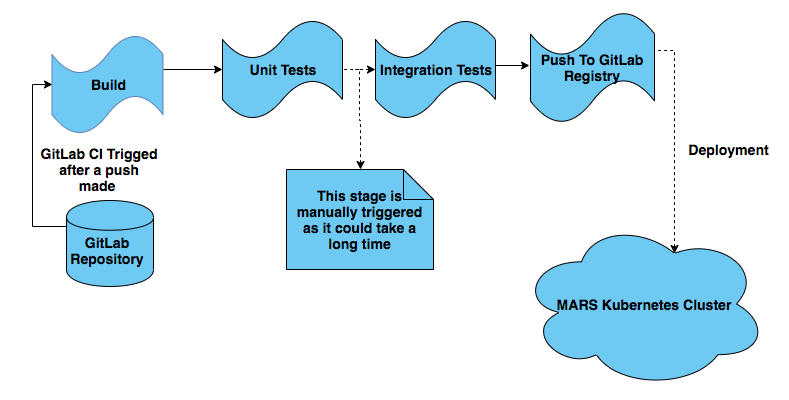
\includegraphics[scale=0.5]{grafiken/CIbuild.png}
    \caption{MARS Continuous Integration Pipeline build}
    \label{fig:CIbuild}
\end{figure}

Figure \ref{fig:CIbuild} presents the Continuous Integration system which is followed by the MARS developer community. This pipeline plays an important role
for the maintenance of the service because the automatic tests are executed here.
The CI\footnote{CI: Continuous Integration} pipeline is triggered as soon as a new commit is pushed to the remote 
GitLab\footnote{https://about.gitlab.com} repository. This builds the Docker image of the service with the new changes. The next step is to
run the unit tests written for the service, which is a mandatory step. Lastly, if the pipeline passes, the docker image is pushed
to the GitLab registry\footnote{https://about.gitlab.com/2016/05/23/gitlab-container-registry/}. If this is successful, then the image can be used in one of 
the MARS Kubernetes clusters, i.e., MARS beta, MARS production environments. 

\section{Unit testing}
These tests are designed to verify the individual components of the software which validates that each unit of the software performs as intended. A White Box
Testing methodology has been applied for the unit testing. This method is used as the internal structure/requirements are known before hand. In this process,
the specific inputs and outputs are predetermined and the tests are ran to verify if the expected output is produced by that input. 

\par
Figure \ref{fig:CIbuild} in the Chapter Requirement Analysis depicts
Unit Testing as an mandatory step for deployment of the Archive service. Running this test with every build process will boost the confidence 
in changing and maintaining the code for the Archive service. The .NET platform offers a lot of unit-testing frameworks 
(e.g. XUnit, Nunit, MSTest/Visual Studio). Nunit is choosen as the preferred the testing framework for this service as it has a good reputation for
fast testing and it is readily integrated the IDE i.e. Rider (JetBrains) used for this work. 

\par
Making stubs, and mocks/fake objects are one of the important steps to do a proper unit testing. This statement can be backed up saying that unit tests are
used to analyze only one module/method. To check only one module the other dependent objects have to faked. The Archive service is designed following the
SOLID \cite{Hotop2015} where the D stands for \textbf{Dependency Inversion Principle} where classes depend upon abstractions i.e. Interfaces not concrete
implementation. The application of this principle has allowed an easy method to fake objects as the depending classes are just abstractions and the concrete 
implementations are injected by the .NET Dependency Injection framework. A framework name as Moq \footnote{https://github.com/Moq/moq4/wiki/Quickstart} is used
which can be used to fake objects i.e.Interfaces and return the desired output from them. 

\begin{lstlisting}[language={[Sharp]C}, caption={Example of faking objects using Moq framework}, captionpos=b,label={lst:moqEg}]
[Fact]
public async Task Archive_CorrectDataId_NoExceptions()
{
    // Arrange
    var fileRepoMock = new Mock<IFileRepo>();
    var fileClientMock = new Mock<IFileClient>();
    // Injecting the mock interfaces 
    var archiveFile = new ArchiveFile(fileRepoMock.Object, fileClientMock.Object);
    var testFileName = "test.zip";
    var testDataId = "4a97bd47-7713-4f4d-89c4-aacf04ae5d20";
    
    // Act
    // Using the Moq framework to return desired output to the method Archive
    fileRepoMock.Setup(m => m.AddFileForProject(It.IsAny<string>(), It.IsAny<byte[]>())).Returns(Task.CompletedTask);
    fileClientMock.Setup(m => m.GetFileAsync(It.IsAny<string>())).ReturnsAsync(new byte[]{1});

    Exception ex = null;
    try
    {
        await archiveFile.Archive(testFileName, testDataId);
    }
    catch (Exception e)
    {
        ex = e;
    }
    
    // Assert
    Assert.Null(ex);
}
\end{lstlisting}

Listing~\ref{lst:moqEg} illustrates an example of unit test done on the Archive method for a file. The Moq framework injects the dependencies and in the setup method
one can return the desired output from the methods. This unit tests verifies if all the dependent methods work as expected.
Following the functional requirements mentioned in Section \ref{section:functionalReq} the unit tests are designed to test if the core logic functions as expected which includes error handling as well.

\subsection{Archive and Retrieve process test}
The unit test designed for these processes are aimed to test the components responsible for each type of resource (See Table \ref{table: archivedMars}) and its 
dependent module. The class overview can be seen from Figure \ref{fig:archiveClassDiagram} and \ref{fig:restoreClass}. Although, the figure does not show all the classes that the archive process is using
but when one sees the attributes that a class is using it will give an good idea of the remaining class under use.

\subsubsection{Test if an background job is enqueued}
For this test, after a successful API request for archiving a project the module should create a background job using Hangfire. This test would check if the
background tasks were created or not. As it is a requirement for the archive process to as a background job it must be ensured that a background job is created 
for a successful request. Listing\ref{lst:hangfireCreate} shows how the test was written to verify the creation of the background job. This process to do this unit
test is mentioned in the Hangfire documentation.

\begin{lstlisting}[language={[Sharp]C}, caption={Hangfire Job creation test}, captionpos=b,label={lst:hangfireCreate}]
[Fact]
public async Task ArchiveProject_SucessfulRun_ShouldBeEnqueued()
{
    // Arrange
    var client = new Mock<IBackgroundJobClient>();
    var iArchiveRepoMock = new Mock<IArchiveStatusLoggerRepo>();
    var mockMarkProject = new Mock<IMarkProject>();
    var mockStatusHandler = new Mock<IBackgroundHandler>();
    var controller = new ArchiveApiController(client.Object, iArchiveRepoMock.Object, mockMarkProject.Object, mockStatusHandler.Object);
    var projectId = Guid.NewGuid().ToString();
    var model = new ArchiveRetrieveStatusModel(){Status = "FINISHED"}; 
    
    // Act
    iArchiveRepoMock.Setup(mo => mo.AddInitialStatus(model)).Returns(Task.CompletedTask);
    mockMarkProject.Setup(mark => mark.MarkAllResourcesForProjectAndGetMarkSession(It.IsAny<string>()))
        .Returns(Task.FromResult(Guid.NewGuid().ToString()));
    iArchiveRepoMock.Setup(mo => mo.GetStatusForId(projectId)).ThrowsAsync(new ResourceNotFoundException(It.IsAny<string>()));

    // Assert
    await controller.ArchiveProject(projectId);
    client.Verify(x => x.Create(
        It.Is<Job>(job => job.Method.Name == "Archive" && (string) job.Args[0] == projectId && job.Args[1] == JobCancellationToken.Null),
        It.IsAny<EnqueuedState>()));

}
\end{lstlisting}

\subsubsection{Return conflict message in case a process for the project is running}
For this test, it checks the denial of a archive or retrieve job creation when a it is in "PROCESSING" state. It is of high priority that this check
for conflict works as expected otherwise there could be cases of unwanted data loss. 

\subsubsection{Exception catch}
For this test, different checks are made in many modules if the expected Exception is caught, in case of an error. Also included is a check for the general
exception class as well. This test will ensure that some method will not just consume an exception when an unexpected error occurs. It is important because if 
the exceptions are not caught it would be very hard to fix bugs if some are introduced in the near future.

\newpage
\begin{lstlisting}[language={[Sharp]C}, caption={Exception catch test example}, captionpos=b,label={lst:exceptionCatch}]
[Fact]
public async Task MarkAllResourceAndGetSessionId_MarkingSvcClientReturnEmpty_ThrowsMarkingFailedException()
{
    // Arrange
    var markingSvcClientMock = new Mock<IMarkingSvcClient>();
    var iArchiveRepoMock = new Mock<IArchiveStatusLoggerRepo>();
    var markProject = new MarkProject(markingSvcClientMock.Object, iArchiveRepoMock.Object);
    
    // Act 
    markingSvcClientMock.Setup(mock => mock.MarkAndGetProjectResources(It.IsAny<string>())).ReturnsAsync(string.Empty);
    
    // Assert
    await Assert.ThrowsAnyAsync<MarkingFailedException>(async () =>
        await markProject.MarkAllResourcesForProjectAndGetMarkSession(It.IsAny<string>()));
}
\end{lstlisting}

\subsubsection{Expected value checks}
For this test, different modules are tested with a mock inputs (e.g. data id, mock models) are made and then the method under test is ran with an 
expected value. These tests are designed to ensure that the methods deliver correct results when a correct input from other modules are received.
These tests would aid the build to discover a faulty implementation according to the requirements mentioned for this work.

\subsubsection{Null or empty checks}
For this test, the different modules are tested against the most famous Null pointer exception in the different modules and how it is handled. This is an important
test case as the archive/retrieve process should still run and terminate accordingly if some resources are null. As an example, during a normal archive run if the result received from
the scenario service  is empty i.e. no scenarios in the project the archive process should not fail due to a null pointer exception rather finish the archive process
as there are no children resources (See Figure \ref{fig:marsDependency}). Listing \ref{lst:scenarisEmpty} shows an example if the scenario client returns a null 
the process does not break but instead the method for archiving scenarios is not triggered. 

\begin{lstlisting}[language={[Sharp]C}, caption={No scenarios added if resource empty}, captionpos=b,label={lst:scenarisEmpty}]
[Fact]
public async Task Archive_NoScenarios_ScenariosNotAdded()
{
    // Arrange
    var scenarioRepoMock = new Mock<IScenarioRepo>();
    var scenarioClientMock = new Mock<IScenarioClient>();
    var markProjectMock = new Mock<IMarkProject>();
    var archiveScenario = new ArchiveScenario(scenarioRepoMock.Object, scenarioClientMock.Object, markProjectMock.Object);
    
    // Act
    markProjectMock.Setup(m => m.GetModelsForResourceType(It.IsAny<string>()))
        .Returns(DependantResourceMock.GetFilteResourceModels("scenario"));
    scenarioClientMock.Setup(m => m.GetScenariosById(It.IsAny<string>()))
        .ReturnsAsync(null);
    await archiveScenario.Archive(It.IsAny<string>());                
    
    // Assert
    scenarioRepoMock.Verify(m => m.AddProjectScenarios(It.IsAny<string>()), Times.Never);
}
\end{lstlisting}

\subsubsection{File read tests}
For this test, the module for reading files from the Synology is tested. To do so dummy files were added (mocking the existence of Synology without 
a network connection) in the build for the unit tests. This test reads the file
and then compares to the expected result. This test is designed to check if the file reading algorithm works as expected. Unfortunately, the module to write the data
could not be tested because when the tests are built they are packed into a .dll file and a write operation is not allowed.

\subsection{Test coverage}
A total of 174 unit test cases were made on the different modules existing in the Archive service at the time of writing this thesis. The total time for running all 
the test cases measured on average is 1m50s. For a proper calculation of the Test coverage by available features in the service Table \ref{table:unitTestCov} gives an short
overview of the type of module and the different features available.

\begin{longtable}{|p{3cm}|p{10cm}|}
    \hline
        \textbf{Modules} & \textbf{Features}\\
    \hline
        Http communication client & File service client, Metadata service client , Scenario service client , Result configuration client, simulation plans client
        , simulation runs client  and simulation results client.\\    
    \hline
        API controller & Archive, Retrieve and background jobs.\\    
    \hline
        Archive & Files, Metadata, Scenario, Result configuration, simulation plans, simulation runs and simulation results.\\  
    \hline
        Retrieve & Files, Metadata, Scenario, Result configuration, simulation plans, simulation runs and simulation results.\\ 
    \hline
        File repositories & Read and Write.\\ 
    \hline
        Utilities & AOP loggers and HTTP helpers.\\ 
    \hline
    \caption{Modules available for unit testing}
    \label{table:unitTestCov} 
\end{longtable}

Out of the 28 different features of the given modules the unit tests were made for 26 of them. This gives a testing coverage for the unit test for about
92\%. Some Test cases could not be carried out due to the complexity of making the tests i.e. AOP\footnote{AOP: Aspect Oriented Programming} loggers, HTTP helpers, File Writers.
\section{Integration Test}
The main aim of this test is to test the communication between the different services that the Archive service is dependent upon. This test is designed in 
such a way that it calls all the endpoints that is used in order to create a simulation run from adding files to running the simulation. As a result of checking
these endpoints it gives an additional benefit of detecting errors introduced from other services in the area of resource creation. As an example, assuming a service
(excluding the Project, User, Marking, and Deletion service)
made some changes which has some bug with resource creation then if the Archive service integration test are executed it would try to recreate the mock resource
and would result in a fail which could then be detected.

\subsection{Challenges}
The Integration Tests are very beneficial to have a more stable system but realizing this test posed really big challenges which took considerably long time with
some constraints. Due to the Microservice architecture of the MARS framework the services are deployed as an independent entity which have their own database.
It was an enormous task to figure out how to combine all these independent services and have them running in a testing environment. The solution to this issue
was to create a multi-container Docker application using Docker-compose. Here, the images of the services required are loaded and the Mongo db database for each
service is seeded. It is also very important for the order for the services and the seeding to loaded in a specific order since the services are dependent upon
each other.  

\begin{lstlisting}[language=docker-compose,caption={Docker compose configuration snippet for Archive service Integration Test}, captionpos=b, breaklines=true,label={code:integCompose}]
archive_svc_tests:
    image: nexus.informatik.haw-hamburg.de/microsoft/dotnet:2.0.0-sdk
    volumes:
      - ../:/mars-archive-svc
    entrypoint:
      - sh
    command:
      - ./mars-archive-svc/IntegrationTests/run_tests.sh
    links:
      - mongodb
      - metadata-svc
      - scenario-svc
      - file-svc
      - reflection-svc
      - resultcfg-svc
      - sim-runner-svc
      - sim-runner
      - mongo-seed
      - result-mongodb
      - result-mongo-seed
      - database-utility-svc
      - marking-svc
    depends_on:
      - mongodb
      - metadata-svc
      - scenario-svc
      - file-svc
      - reflection-svc
      - resultcfg-svc
      - sim-runner-svc
      - sim-runner
      - mongo-seed
      - result-mongodb
      - result-mongo-seed
      - database-utility-svc
      - marking-svc
\end{lstlisting}      

Listing~\ref{code:integCompose} shows a snippet of the docker compose file for running the Integration Test. The depends\_on attribute for the archive service
has many services in it. This means the archive\_svc\_test is waiting for the other services to load and the mongodb to be seeded with mock data. Unfortunately,
since the Project service does not use Mongodb but instead Postgres Sql as a database for some unknown reason the synchronization of the seeding of the data
did not succeed and therefore the tests could not be ran. The
Marking service and Deletion service endpoints that the Archive service uses have a dependency with the Project service  which resulted as a unsuccessful test
for them. Although, it is a point of interest in the future to investigate to figure out the reason for this and complete the whole test.

\subsection{Correctness of received data}
For this test, the GET endpoints of the services were tested. A dummy model for the data which the Archive service expects is compared to the result
form the GET endpoints. This check would aid to verify if the services return a data model which the service. If any changes to the other services
related to the data model is made this test would detect it. 

\subsection{Correctness for uploading data}
For this test, the POST, PUT and PATCH endpoints were tested. It is designed to verify during the restoring process if the expected data model 
is still compatible with the services or if there is some error introduced after a new change. The process is conducted by uploading the 
data models using the mentioned endpoints and in return expecting a success status.

\subsection{Correctness of response}
This test is designed to check the interface of the API provided by the other services. This check would aid to validate if the API of the
service returns a correct status as described by their Swagger interface. As an example, while posting a scenario in the scenario service if the
name and the data id of the model is already existing an conflict status code will be returned by the request. Therefore, for this example an existing
model would be uploaded and the test would verify if an conflict status is returned. Likewise, the other responses are verified by this test. 

\subsection{Integration with the Database}
This test is designed to test if a proper integration between the Mongodb and Archive service is maintained. The Archive service stores vital metadata
which gives the client information about the status of the job and many other data that it needs. This check verifies the correctness of the read and write 
operations done with the Database. 

\subsection{Test Coverage}
A total of 81 tests were made which would aid in verifying the integration of the Archive service with the dependent services and the database. The 
total time for running the test measured at the time of writing the thesis is on average 7m38s. Table \ref{table:MARS Resource Hierarchy Service Overview}
mentions the services that the archive service has dependency towards and 6 out of 9 services are being tested for the integration test. Among the total services 
which were supposed to be tested only 67\%  were carried out. It is a point of interest in the future to complete fulfill these requirements which would boost the
reliability of the Archive service. 

\section{System Test}
This test verifies the requirements mentioned in Section \ref{section:functionalReq} by performing manual GUI tests. System test are manual tests
which ensure the correct behavior of the system.

\subsection{Successful archive process start}
For this test, it is verified whether the archive process can be started from the MARS Teaching GUI with the precondition that no other process
for this project is running. One Wolves and Sheep model is uploaded with other resources i.e. scenario, result configuration,
simulation plan, simulation run and simulation result. As this test is to verify the successful execution of the process only one of each resources
were uploaded and checked.

\subsection{Archive with a More Complex Model}
For this test, the Kruger National Park (KNP) model is used to test instead of the Wolves and Sheep because the KNP is more complex because it requires more layers
i.e. GIS, Timeseries, Geopotential layers. The successful archive of this model with all its resources i.e. scenario, result configuration, simulation plan, simulation run
and simulation results were verified. 

\subsection{Successful Data Archive in Synology}
For this test, the Synology drive where the archives were supposed to be uploaded were verified. The successful archive process of the Wolves and Sheep model
was correctly stored in the archive folder inside the drive.

\subsection{Successful Retrieve Process Start}
For this test, it is verified if the retrieve process could be successfully started from the MARS Teaching GUI when no process for the project is running.
Both the KNP and Wolves and Sheep models with its resources were restored back to the system with all its resources. 

\subsection{Correctness of the Restored Project}
For this test, it is verified if the retrieved data are the same as from the archive. Also, a check is done whether the restored files can be used in the active system
to produce further results (e.g. a simulation was ran from the restored simulation plan, a new scenario is created from the model).

\subsection{Fault-Tolerance Test}
For this test, a intentional error is created to verify if the implemented strategy for fault tolerance is executed. A successful verification for this
strategy was checked. Also a check was done by removing the server from the cluster while a job are being processed. This checked verified that the Archive service
would restart the job in case of sudden failure after the server has be revived. This is the case only if the defined number of retires are not exceeded.
\section{Performance Test}
This test verifies the performance metrics of the Archive service analyzing different numbers of files, file sizes and archive strategies.

\subsection{Archive performance}
For this test, the an archive process is executed and repeated 4 times to get an average general performance overview. Figure \ref{fig:archivePerformance} illustrates a bar diagram for running an archive process (zipped simulation results) with 7 files, 2 scenarios, 2 result configurations, 2 simulation plans
and 12 simulation runs and results. The results seen in the figure shows that it took about 34.9 s on average to run this process. It is also to be noted that the
simulation results are zipped making their total size about 86 Mb. Figure \ref{fig:archivePerformanceUn} shows the archive process of ths same project without 
compressing the simulation results and it can be seen that the file sizes for the uncompressed process is significantly higher in contrast to the compressed
process with file size on avg about 683 Mb and 43s processing time.

\begin{figure}[H]
    \centering 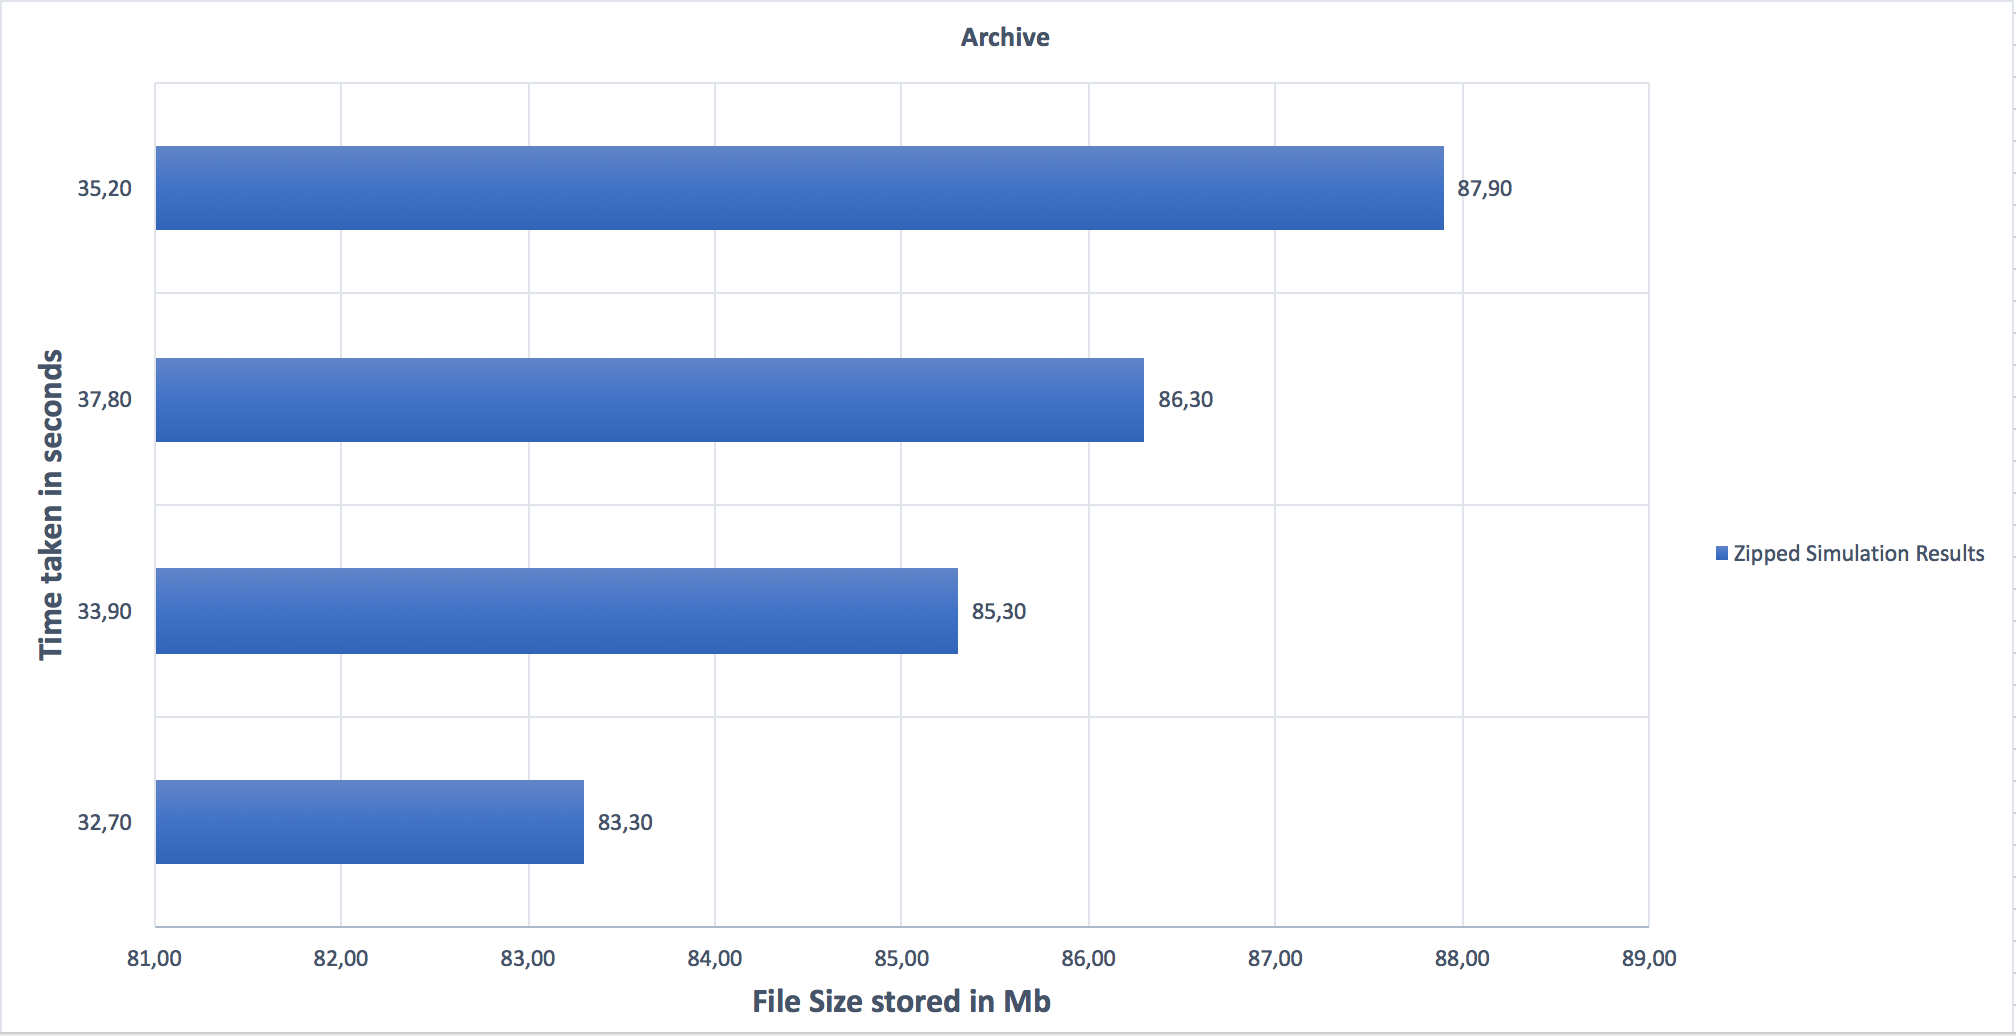
\includegraphics[scale=0.5]{grafiken/archiveZip.png}
    \caption{Overall performance of the archive process (compressed simulation results)}
    \label{fig:archivePerformance}
\end{figure}

\begin{figure}[H]
    \centering 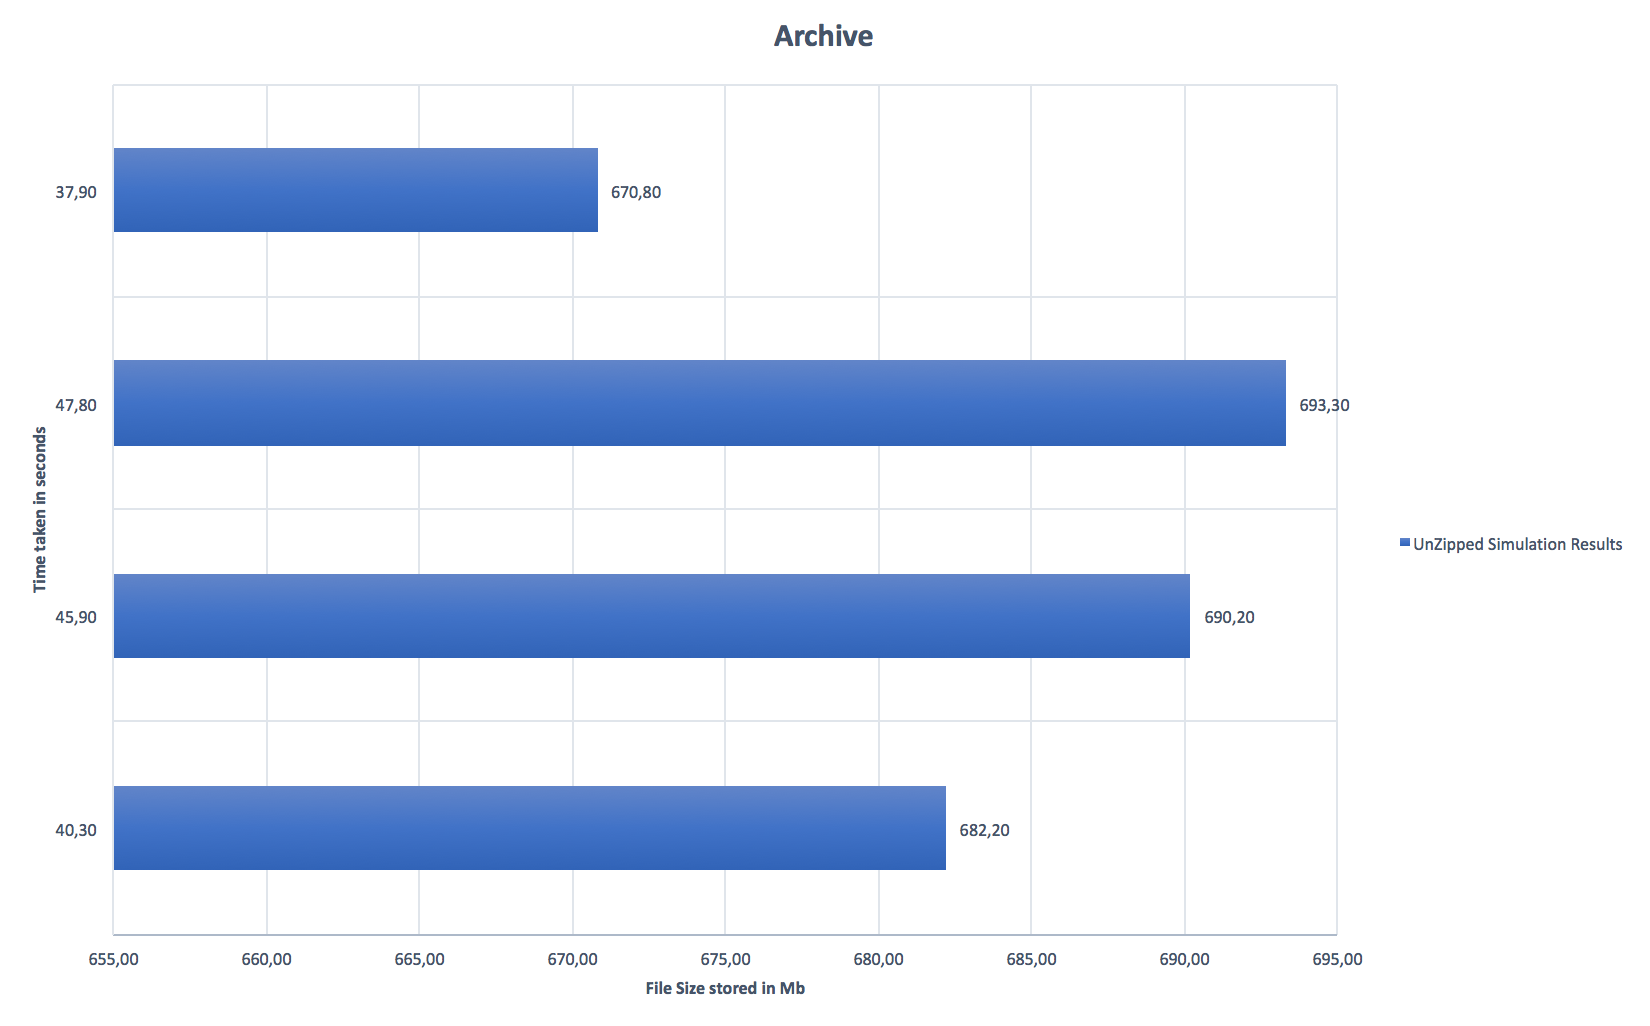
\includegraphics[scale=0.5]{grafiken/archiveUnzip.png}
    \caption{Overall performance of the archive process (uncompressed simulation results)}
    \label{fig:archivePerformanceUn}
\end{figure}

Unfortunately simulation results with larger file sizes could not be tested as no such simulation results was available at the moment but with this metrics it can be said that
for smaller file sizes it is a better choice to compress the simulation data while archiving it since there is a significant data volume save and the time taken for the
archive does not differ by much.   

\subsection{Retrieve Performance}
For this test, the same project that was archived is being restored to analyze the performance of the retrieve process. Figure \ref{fig:restorePerformance} illustrates
the results of the retrieve process with the compressed simulation results which takes 4.3 mins on average. Figure \ref{fig:restorePerformanceUn} illustrates the
results of the retrieve process using the uncompressed simulation results which took on average of 4 mins. It is seen that the for projects having their total file
size similar to the analyzed one is benefited by using the compression feature.

\begin{figure}[H]
    \centering 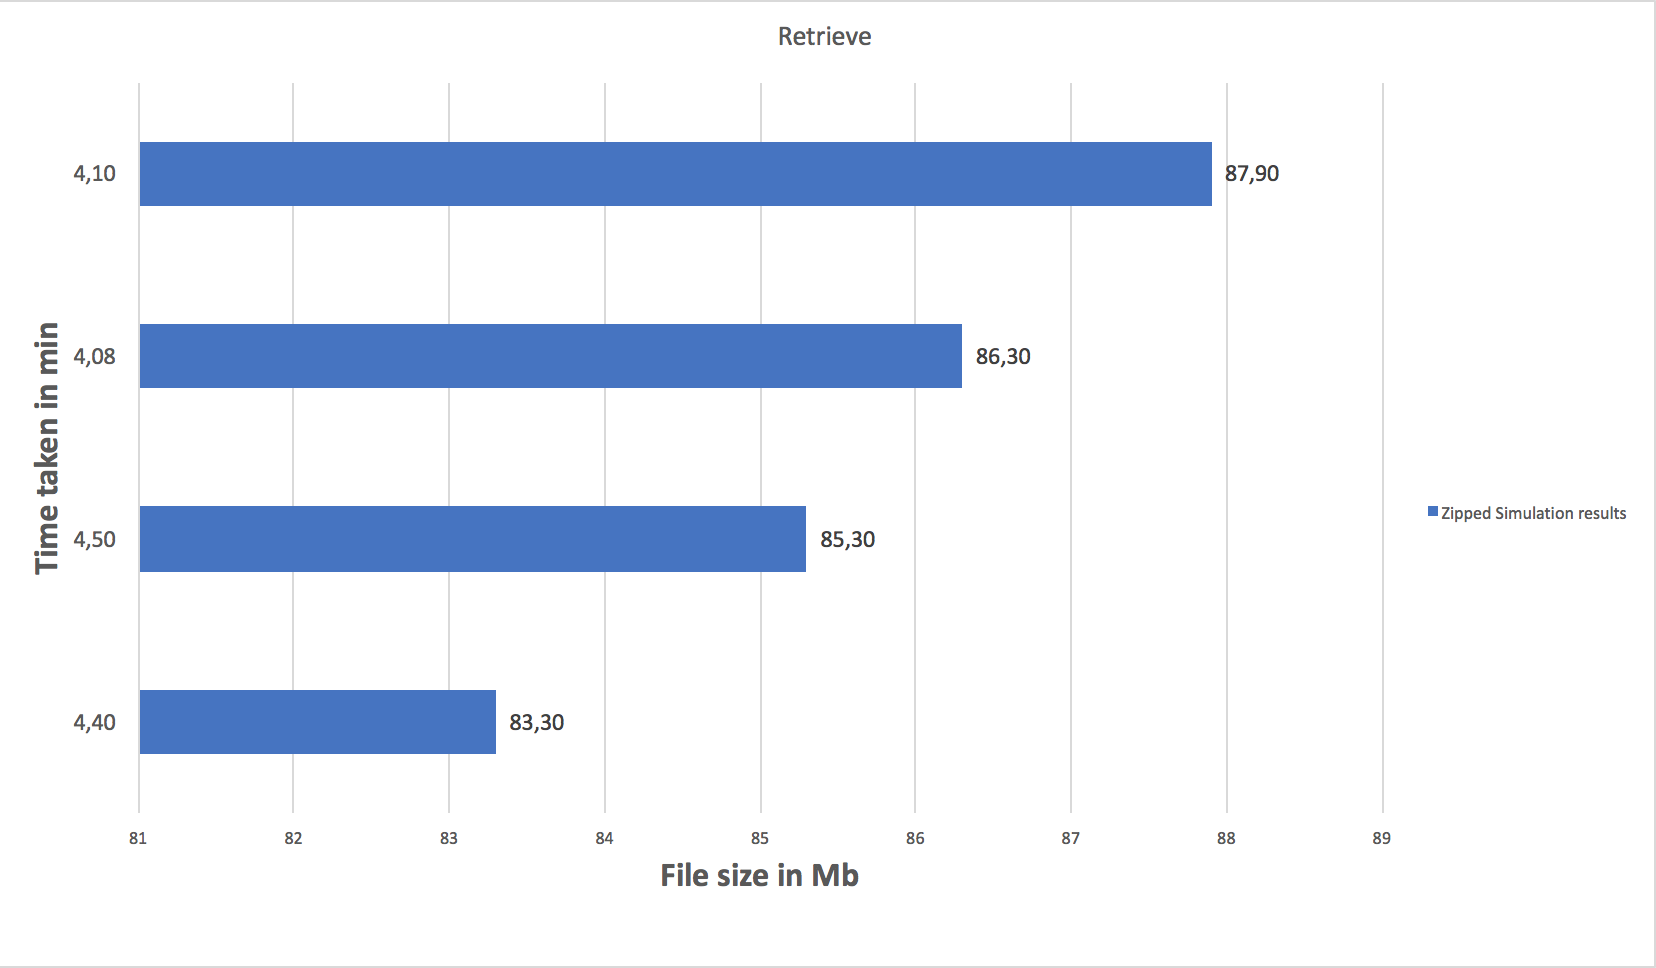
\includegraphics[scale=0.7]{grafiken/retrieveZip.png}
    \caption{Overall performance of the retrieve process (compressed simulation results)}
    \label{fig:restorePerformance}
\end{figure}

\begin{figure}[H]
    \centering 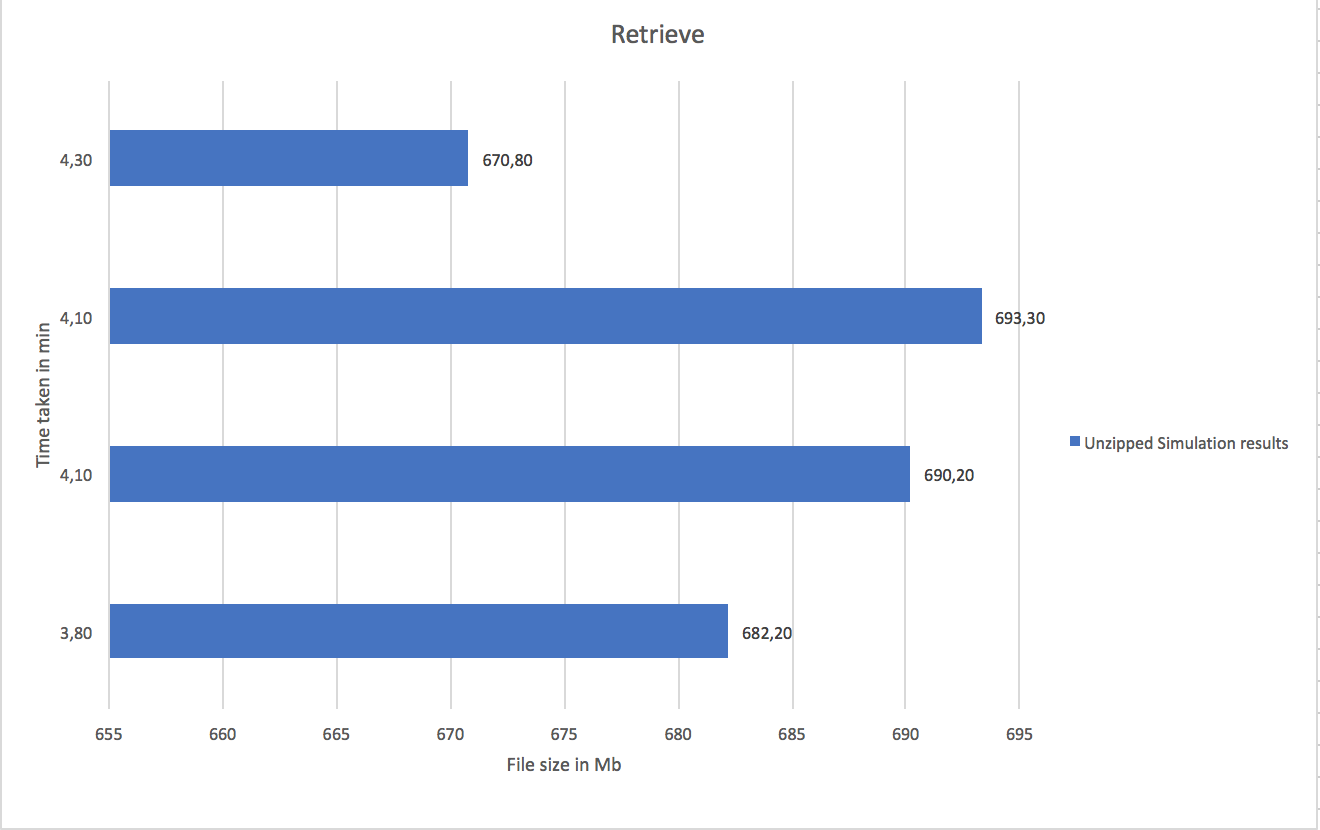
\includegraphics[scale=0.7]{grafiken/retrieveUnzip.png}
    \caption{Overall performance of the retrieve process (uncompressed simulation results)}
    \label{fig:restorePerformanceUn}
\end{figure}